%
% Copyright 2018 Joel Feldman, Andrew Rechnitzer and Elyse Yeager.
% This work is licensed under a Creative Commons Attribution-NonCommercial-ShareAlike 4.0 International License.
% https://creativecommons.org/licenses/by-nc-sa/4.0/
%
\questionheader{ex:s3.6.3}


%%%%%%%%%%%%%%%%%%
\subsection*{\Conceptual}
%%%%%%%%%%%%%%%%%%

\begin{Mquestion}
On the graph below, mark the intervals where $f''(x)>0$ (i.e. $f(x)$ is concave up) and where $f''(x)<0$ (i.e. $f(x)$ is concave down).
\begin{center}
\begin{tikzpicture}
\YEaxis{6}{4}
\draw[thick] plot[domain=-6:-2](\x,{exp(\x+2)+1});
\draw[thick] plot[domain=-2:4](\x,{cos(\x*.785 r)+2});
\draw[thick] plot[domain=0:2](\x+4,{3*cos(\x*.785 r)-2});
\end{tikzpicture}
\end{center}
\end{Mquestion}
\begin{hint}
There are two intervals where the function is concave up, and two where it is concave down.
\end{hint}
\begin{answer}
\begin{center}
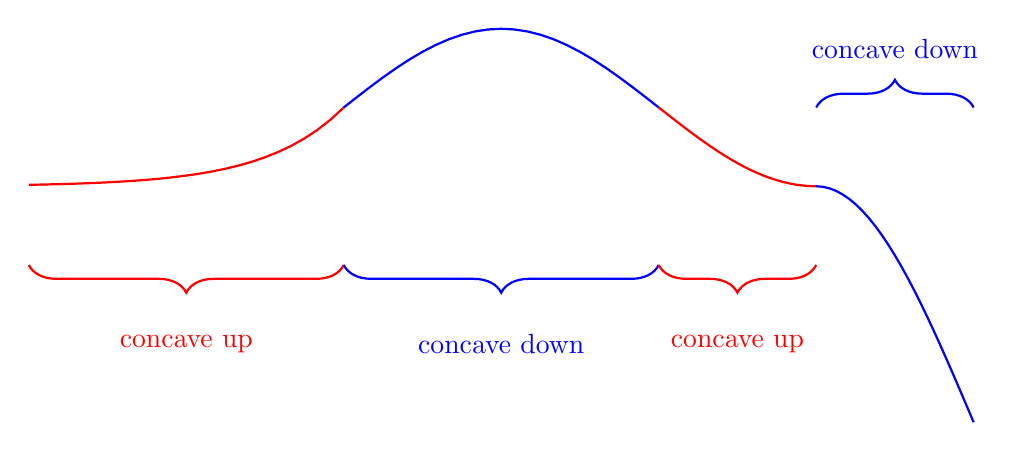
\begin{tikzpicture}
\YEaxis{6}{4}
\draw[thick, red] plot[domain=-6:-2](\x,{exp(\x+2)+1});
\draw[thick, blue] plot[domain=-2:2](\x,{cos(\x*.785 r)+2});
\draw[thick, red] plot[domain=2:4](\x,{cos(\x*.785 r)+2});
\draw[thick, blue] plot[domain=0:2](\x+4,{3*cos(\x*.785 r)-2});
\draw[thick, red, decorate, decoration={brace, amplitude=10pt, mirror}]
(-6,0)--(-2,0);
\draw[red] (-4,-1) node{concave up};
\draw[thick, blue, decorate, decoration={brace, amplitude=10pt, mirror}]
(-2,0)--(2,0);
\draw[blue] (0,-1) node{concave down};
\draw[thick, red, decorate, decoration={brace, amplitude=10pt, mirror}]
(2,0)--(4,0);
\draw[red] (3,-1) node{concave up};
\draw[thick, blue, decorate, decoration={brace, amplitude=10pt}]
(4,2)--(6,2);
\draw[blue] (5,2.75) node{concave down};
\end{tikzpicture}
\end{center}
\end{answer}
\begin{solution}
\begin{center}
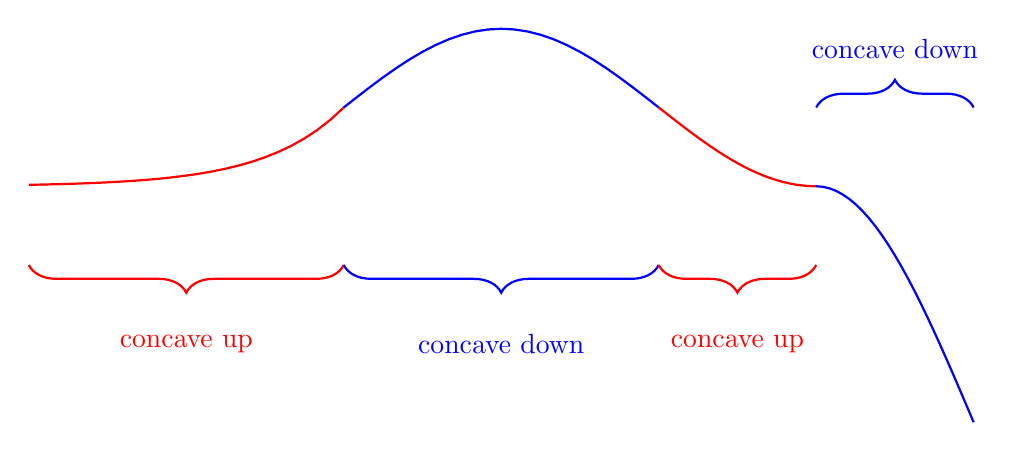
\begin{tikzpicture}
\YEaxis{6}{4}
\draw[thick, red] plot[domain=-6:-2](\x,{exp(\x+2)+1});
\draw[thick, blue] plot[domain=-2:2](\x,{cos(\x*.785 r)+2});
\draw[thick, red] plot[domain=2:4](\x,{cos(\x*.785 r)+2});
\draw[thick, blue] plot[domain=0:2](\x+4,{3*cos(\x*.785 r)-2});
\draw[thick, red, decorate, decoration={brace, amplitude=10pt, mirror}]
(-6,0)--(-2,0);
\draw[red] (-4,-1) node{concave up};
\draw[thick, blue, decorate, decoration={brace, amplitude=10pt, mirror}]
(-2,0)--(2,0);
\draw[blue] (0,-1) node{concave down};
\draw[thick, red, decorate, decoration={brace, amplitude=10pt, mirror}]
(2,0)--(4,0);
\draw[red] (3,-1) node{concave up};
\draw[thick, blue, decorate, decoration={brace, amplitude=10pt}]
(4,2)--(6,2);
\draw[blue] (5,2.75) node{concave down};
\end{tikzpicture}
\end{center}
In the graph above, the concave-up sections are marked in red. These are where the graph has an increasing derivative; equivalently, where the graph lies above its tangent lines; more descriptively, where it curves like a smiley face.

Concave-down sections are marked in blue. These are where the graph has a decreasing derivative; equivalently, where the graph lies below its tangent lines; more descriptively, where it curves like a frowney face.
\end{solution}



\begin{Mquestion}
Sketch a curve that is:
\begin{itemize}
\item concave up when $|x|>5$,
\item concave down when $|x|<5$,
\item increasing when $x<0$, and
\item decreasing when $x>0$.
\end{itemize}
\end{Mquestion}
\begin{hint}
Try allowing your graph to have horizontal asymptotes. For example, let the function get closer and closer to the $x$-axis (or another horizontal line) without touching it.
\end{hint}
\begin{answer}
\begin{center}
\begin{tikzpicture}
\YEaaxis{6}{6}{1}{4}
\draw[thick] plot[domain=-3:0] (\x-3,{exp(\x)});
\draw[thick] plot[domain=0:3] (\x+3,{exp(-\x)});
\draw[thick] plot[domain=-3:3] (\x,{cos(\x*0.523 r)/0.523+1});
\YExcoord{-3}{-5}
\YExcoord{3}{5}
\end{tikzpicture}
\end{center}
\end{answer}
\begin{solution}
The most basic shape of the graph is given by the last two bullet points:
\begin{center}
\begin{tikzpicture}
\YEaaxis{6}{6}{1}{4}
\draw[thick, <->] (-6,1)--(0,3)--(6,1);
\YExcoord{-3}{-5}
\YExcoord{3}{5}
\end{tikzpicture}
\end{center}
The curve is concave down over the interval $(-5,5)$, so let's give it a frowney-face curvature there.
\begin{center}
\begin{tikzpicture}
\YEaaxis{6}{6}{1}{4}
\draw[thick] plot[domain=-3:3] (\x,{cos(\x*0.523 r)/0.523+1});
\draw[thick] (-6,-.25)--(-3,1) (3,1)--(6,-.25);
\YExcoord{-3}{-5}
\YExcoord{3}{5}
\end{tikzpicture}
\end{center}
Finally, when $x>5$ or $x<-5$, our curve should be concave up, so let's give it smiley-face curvature there, without changing its basic increasing/decreasing shape.
\begin{center}
\begin{tikzpicture}
\YEaaxis{6}{6}{1}{4}
\draw[thick] plot[domain=-3:0] (\x-3,{exp(\x)});
\draw[thick] plot[domain=0:3] (\x+3,{exp(-\x)});
\draw[thick] plot[domain=-3:3] (\x,{cos(\x*0.523 r)/0.523+1});
\YExcoord{-3}{-5}
\YExcoord{3}{5}
\end{tikzpicture}
\end{center}
This finishes our sketch.
\end{solution}


\begin{question}\label{s3.6.3converse}
Suppose $f(x)$ is a function whose second derivative exists and is continuous for all real numbers.

True or false: if $f''(3)=0$, then $x=3$ is an inflection point of $f(x)$.

Remark: compare to Question~\ref{s3.6.3IVT}
\end{question}
\begin{hint}
Consider $f(x)=(x-3)^4$.
\end{hint}
\begin{answer}
In general, false.
\end{answer}
\begin{solution}
An inflection point is where the concavity of a function changes. It is possible that $x=3$ is an inflection point, but it is also possible that is not. So, the statement is false, in general.

For example, let $f(x)=(x-3)^4$. Since $f(x)$ is a polynomial, all its derivatives exist and are continuous. $f''(x)=12(x-3)^2$, so $f''(3)=0$. However, since $f''(x)$ is something squared, it is never negative, so $f(x)$ is never concave down. Since $f(x)$ is never concave down, it never changes concavity, so it has no inflection points.

Remark: finding inflection points is somewhat reminiscent of finding local extrema. To find local extrema, we first find all critical and singular points, since local extrema can only occur there or at endpoints. Then, we have to figure out which critical and singular points are actually local extrema. Similarly, if you want to find inflection points, start by finding where $f''(x)$ is zero or non-existant, because inflection points can only occur there (see Question~\ref{s3.6.3IVT}). Then, you still have to check whether those points are actually inflection points.
\end{solution}
%%%%%%%%%%%%%%%%%%
\subsection*{\Procedural}
%%%%%%%%%%%%%%%%%%


\begin{Mquestion}[1997D]
Find all inflection points for the graph of $f(x)=3x^5-5x^4+13x$.
\end{Mquestion}
\begin{answer}
$x=1,\ y=11$
\end{answer}
\begin{solution}
Inflection points occur where $f''(x)$ changes sign. Since $f(x)$ is a polynomial, its first and second derivatives exist everywhere, and are themselves polynomials. In particular,
\begin{align*}f(x)&=3x^5-5x^4+13x\\
f'(x)&=15x^4-20x^3+13\\
f''(x)&=60x^3-60x^2=60x^2(x-1)
\end{align*}
The second derivative is negative for $x<1$ and positive for $x>1$. Thus
the concavity changes between concave up and concave down at
{$x=1,\ y=11$}.

This is the only inflection point. It is true that $f''(0)=0$, but for values of $x$ both a little larger than and a little smaller than 0, $f''(x)<0$, so the concavity does not change at $x=0$.
\end{solution}


%%%%%%%%%%%%%%%%%%
\subsection*{\Application}
%%%%%%%%%%%%%%%%%%

\Instructions{Questions~\ref{s3.6.3proof1} through \ref{s3.6.3IVT} ask you to show that certain things are true. Give a clear explanation using concepts and theorems from the CLP-1 text.}

\begin{Mquestion}[1997A]\label{s3.6.3proof1}
Let
\[f(x)=\frac{x^5}{20}+\frac{5x^3}{6}-10x^2+500x+1000\]
Show that $f(x)$ has exactly one inflection point.
\end{Mquestion}
\begin{hint}
You must show it has at least one inflection point (try the Intermediate Value Theorem), and at most one inflection point (consider whether the second derivative is increasing or decreasing).
\end{hint}
\begin{answer}
Let \[g(x)=f''(x)=x^3+5x-20.\] Then $g'(x)=3x^2+5$, which is always positive. That means $g(x)$ is strictly increasing for all $x$. So, $g(x)$ can change signs once, from negative to positive, but it can never change back to negative. An inflection point of $f(x)$ occurs when $g(x)$ changes signs. So, $f(x)$ has \emph{at most one} inflection point.

Since $g(x)$ is continuous, we can apply the Intermediate Value Theorem to it. Notice
$g(3)>0$ while $g(0)<0$. By the IVT, $g(x)=0$ for at least one $x \in (0,3)$. Since $g(x)$ is strictly increasing, at the point where $g(x)=0$, $g(x)$ changes from negative to positive. So, the concavity of $f(x)$ changes. Therefore, $f(x)$ has \emph{at least one} inflection point.

Now that we've shown that $f(x)$ has at most one inflection point, and at least one inflection point, we conclude it has exactly one inflection point.\end{answer}
\begin{solution}
In order to show that $f(x)$ has \emph{exactly one} inflection point, we will show that is has \emph{at least one}, and \emph{no more than one}.

Let \[g(x)=f''(x)=x^3+5x-20.\] Then $g'(x)=3x^2+5$, which is always positive. That means $g(x)$ is strictly increasing for all $x$. So, $g(x)$ can change signs once, from negative to positive, but it can never change back to negative. An inflection point of $f(x)$ occurs when $g(x)$ changes signs. So, $f(x)$ has at most one inflection point. (At this point, we don't know that $f(x)$ has any inflection points: maybe $g(x)$ is always positive.)

Since $g(x)$ is continuous, we can apply the Intermediate Value Theorem to it. Notice
$g(3)>0$ while $g(0)<0$. By the IVT, $g(x)=0$ for at least one $x \in (0,3)$. Since $g(x)$ is strictly increasing, at the point where $g(x)=0$, $g(x)$ changes from negative to positive. So, the concavity of $f(x)$ changes. Therefore, $f(x)$ has at least one inflection point.

Now that we've shown that $f(x)$ has at most one inflection point, and at least one inflection point, we conclude it has exactly one inflection point.
\end{solution}



\begin{Mquestion}[1996D]
Let $f(x)$ be a function whose first two derivatives exist everywhere, and $f''(x)>0$ for all $x$.
\begin{enumerate}[(a)]
 \item\label{s3.6interval1} Show that $f(x)$ has at most one critical point and that any critical point is an absolute minimum for $f(x)$.
  \item\label{s3.6interval2} Show that the maximum value of $f(x)$ on any finite interval
occurs at one of the endpoints of the interval.
\end{enumerate}
\end{Mquestion}
\begin{hint}
Use \eqref{s3.6interval1} in
proving \eqref{s3.6interval2}.
\end{hint}
\begin{answer}
\eqref{s3.6interval1}
Let
\[g(x)=f'(x)\]
Then $f''(x)$ is the derivative of $g(x)$. Since $f''(x)>0$ for all $x$, $g(x)=f'(x)$ is strictly increasing
for all $x$.
In other words, if $y>x$ then $g(y)>g(x)$.

Suppose $g(x)=0$. Then for every $y$ that is larger than $x$, $g(y)>g(x)$, so $g(y) \neq 0$. Similarly, for every $y$ that is smaller than $x$, $g(y)<g(x)$, so $g(y) \neq 0$. Therefore, $g(x)$ can only be zero for at most one value of $x$. Since $g(x)=f'(x)$, that means $f(x)$ can have at most one critical point.

Suppose $f'(c)=0$. Since
$f'(x)$ is a strictly increasing function, $f'(x)<0$ for all $x<c$ and $f'(x)>0$ for all $x>c$.
\begin{center}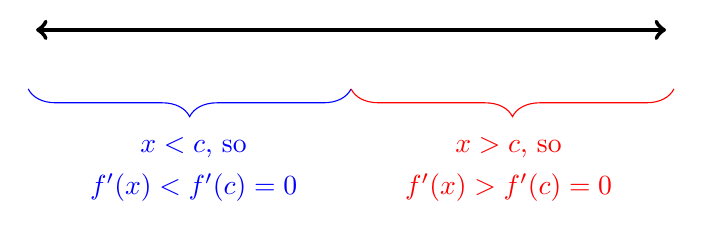
\begin{tikzpicture}
\draw[ultra thick, <->] (-4,0)--(4,0);
\YExcoord{0}{c}
\draw[blue, decorate, decoration={brace, mirror, amplitude=10pt}] (-4.1,-.75)--(0,-.75);
\draw[blue] (-2,-1.5) node{$x<c$, so};
\draw[blue] (-2,-2) node{$f'(x)<f'(c)=0$};
\draw[red, decorate, decoration={brace, amplitude=10pt}] (4.1,-.75)--(0,-.75);
\draw[red] (2,-1.5) node{$x>c$, so};
\draw[red] (2,-2) node{$f'(x)>f'(c)=0$};
\end{tikzpicture}\end{center}

Then $f(x)$ is decreasing for $x<c$ and increasing for $x>c$.
So $f(x)>f(c)$ for all $x\neq c$.

\begin{center}\begin{tikzpicture}
\draw[ultra thick, <->] (-4,0)--(4,0);
\YExcoord{0}{c}
\draw[blue, decorate, decoration={brace, mirror, amplitude=10pt}] (-4.1,-.75)--(0,-.75);
\draw[blue] (-2,-1.5) node{$f(x)$ decreasing, so};
\draw[blue] (-2,-2) node{$f(x)>f(c)$};
\draw[red, decorate, decoration={brace, amplitude=10pt}] (4.1,-.75)--(0,-.75);
\draw[red] (2,-1.5) node{$f(x)$ increasing, so};
\draw[red] (2,-2) node{$f(x)>f(c)$};
\draw[thick, dashed] (-4,3)--(0,1)--(4,3) node[right]{$y=f(x)$};
\draw[blue] (-2,2) node[vertex]{};
\draw (0,1) node[vertex]{};
\draw[red] (2,2) node[vertex]{};
\color{blue}\YExcoord{-2}{x<c}
\color{red}\YExcoord{2}{x>c}
\end{tikzpicture}\end{center}
 Since $f(x)>f(c)$ for
all $x\ne c$, so $c$ is an absolute minimum for $f(x)$.

\eqref{s3.6interval2}
We know that the maximum over an interval occurs at an endpoint,
a critical point, or a singular point.
\begin{itemize}
\item  Since $f'(x)$ exists everywhere, there are no singular points.
\item If the maximum were achieved at a critical point, that critical point would
have to provide both the absolute maximum and the absolute minimum (by part (a)).
So, the function would have to be a constant and consequently could not have
a nonzero second derivative. So the maximum is not at a critical point.
\end{itemize}
That leaves only the endpoints of the interval.
\end{answer}
\begin{solution}
\eqref{s3.6interval1}
Let
\[g(x)=f'(x)\]
Then $f''(x)$ is the derivative of $g(x)$. Since $f''(x)>0$ for all $x$, $g(x)=f'(x)$ is strictly increasing
for all $x$.
In other words, if $y>x$ then $g(y)>g(x)$.

Suppose $g(x)=0$. Then for every $y$ that is larger than $x$, $g(y)>g(x)$, so $g(y) \neq 0$. Similarly, for every $y$ that is smaller than $x$, $g(y)<g(x)$, so $g(y) \neq 0$. Therefore, $g(x)$ can only be zero for at most one value of $x$. Since $g(x)=f'(x)$, that means $f(x)$ can have at most one critical point.

Suppose $f'(c)=0$. Since
$f'(x)$ is a strictly increasing function, $f'(x)<0$ for all $x<c$ and $f'(x)>0$ for all $x>c$.
\begin{center}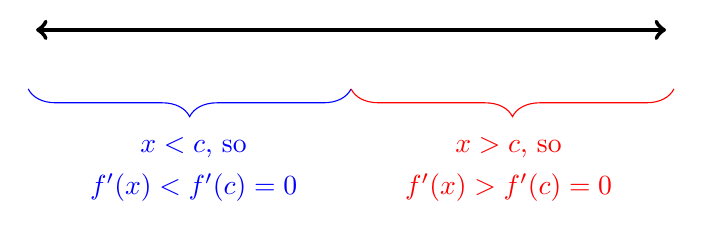
\begin{tikzpicture}
\draw[ultra thick, <->] (-4,0)--(4,0);
\YExcoord{0}{c}
\draw[blue, decorate, decoration={brace, mirror, amplitude=10pt}] (-4.1,-.75)--(0,-.75);
\draw[blue] (-2,-1.5) node{$x<c$, so};
\draw[blue] (-2,-2) node{$f'(x)<f'(c)=0$};
\draw[red, decorate, decoration={brace, amplitude=10pt}] (4.1,-.75)--(0,-.75);
\draw[red] (2,-1.5) node{$x>c$, so};
\draw[red] (2,-2) node{$f'(x)>f'(c)=0$};
\end{tikzpicture}\end{center}

Then $f(x)$ is decreasing for $x<c$ and increasing for $x>c$.
So $f(x)>f(c)$ for all $x<c$ and $f(x)>f(c)$ for all $x>c$.

\begin{center}\begin{tikzpicture}
\draw[ultra thick, <->] (-4,0)--(4,0);
\YExcoord{0}{c}
\draw[blue, decorate, decoration={brace, mirror, amplitude=10pt}] (-4.1,-.75)--(0,-.75);
\draw[blue] (-2,-1.5) node{$f(x)$ decreasing, so};
\draw[blue] (-2,-2) node{$f(x)>f(c)$};
\draw[red, decorate, decoration={brace, amplitude=10pt}] (4.1,-.75)--(0,-.75);
\draw[red] (2,-1.5) node{$f(x)$ increasing, so};
\draw[red] (2,-2) node{$f(x)>f(c)$};
\draw[thick, dashed] (-4,3)--(0,1)--(4,3) node[right]{$y=f(x)$};
\draw[blue] (-2,2) node[vertex]{};
\draw (0,1) node[vertex]{};
\draw[red] (2,2) node[vertex]{};
\color{blue}\YExcoord{-2}{x<c}
\color{red}\YExcoord{2}{x>c}
\end{tikzpicture}\end{center}
 We have concluded that $f(x)>f(c)$ for
all $x\ne c$, so $c$ is an absolute minimum for $f(x)$.

\eqref{s3.6interval2}
We know that the maximum over an interval occurs at an endpoint,
at a critical point, or at a singular point.
\begin{itemize}
\item  Since $f'(x)$ exists everywhere, there are no singular points.
\item If the maximum were achieved at a critical point, that critical point would
have to provide both the absolute maximum and the absolute minimum (by part a).
So, the function would have to be a constant and consequently could not have
a nonzero second derivative. So the maximum is not at a critical point.
\end{itemize}
That leaves only the endpoints of the interval.

%Remark: The question should
%have explicitly told you that $f'$ exists everywhere -- otherwise the maximum
%need not occur at an end point! For example, $f(x)=-x^{2/3}$ has
%$f'(x)=-\frac{2}{3}x^{-1/3}$ and $f''(x)=\frac{2}{9}x^{-4/3}
%=\frac{2}{9}\big(x^{-2/3}\big)^2>0$. But $f(x)$ has its maximum at $x=0$
%because $f(0)=0$ and $f(x)=-\big(x^{1/3}\big)^2<0$ for all $x\ne 0$.
%
%\begin{center}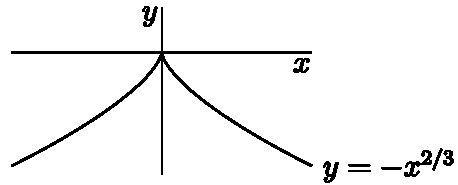
\includegraphics{graphE10}\end{center}
\end{solution}


\begin{question}\label{s3.6.3IVT}
Suppose $f(x)$ is a function whose second derivative exists and is continuous for all real numbers, and $x=3$ is an inflection point of $f(x)$. Use the Intermediate Value Theorem to show that $f''(3)=0$.

Remark: compare to Question~\ref{s3.6.3converse}.
\end{question}
\begin{hint}
Since $x=3$ is an inflection point, we know the concavity of $f(x)$ changes at $x=3$.
That is, there is some interval around 3, with endpoints $a$ and $b$, such that
\begin{itemize}
\item \textcolor{blue}{$f''(a)<0$ and $f''(x)<0$ for every $x$ between $a$ and 3,} and
\item \textcolor{red}{$f''(b)>0$ and $f''(x)>0$ for every $x$ between $b$ and 3.}
\end{itemize}
Use the IVT to show that $f''(x)=3$ for \emph{some} $x$ between $a$ and $b$; then show that this value of $x$ can't be anything \emph{except} $x=3$.
\end{hint}
\begin{answer}
If $x=3$ is an inflection point, then the concavity of $f(x)$ changes at $x=3$. That is, there is some interval strictly containing 3, with endpoints $a$ and $b$, such that
\begin{itemize}
\item \textcolor{blue}{$f''(a)<0$ and $f''(x)<0$ for every $x$ between $a$ and 3,} and
\item \textcolor{red}{$f''(b)>0$ and $f''(x)>0$ for every $x$ between $b$ and 3.}
\end{itemize}

Since $f''(a)<0$ and $f''(b)>0$, and since $f''(x)$ is continuous, the Intermediate Value Theorem tells us that there exists some $x$ strictly between $a$ and $b$ with $f''(x)=0$. So, we know $f''(x)=0$ somewhere between $a$ and $b$. The question is, where exactly could that be?

\begin{itemize}
\item $f''(x)<0$ (and hence $f''(x) \neq 0$) for all $x$ between $a$ and 3
\item $f''(x)>0$ (and hence $f''(x) \neq 0$)  for all $x$ between $b$ and 3
\item So, any number between $a$ and $b$ that is not 3 has $f''(x)\neq 0$.
\end{itemize}
So, $x=3$ is the only possible place between $a$ and $b$ where $f''(x)$ could be zero. Therefore, $f''(3)=0$.
\end{answer}
\begin{solution}
If $x=3$ is an inflection point, then the concavity of $f(x)$ changes at $x=3$. That is, there is some interval strictly containing 3, with endpoints $a$ and $b$, such that
\begin{itemize}
\item \textcolor{blue}{$f''(a)<0$ and $f''(x)<0$ for every $x$ between $a$ and 3,} and
\item \textcolor{red}{$f''(b)>0$ and $f''(x)>0$ for every $x$ between $b$ and 3.}
\end{itemize}
Remark: we are leaving unknown whether $a<3<b$ or $b<3<a$. Since we don't know whether $f(x)$ changes from concave up to concave down, or from concave down to concave up, by remaining vague we cover both cases.
\vspace{5mm}
\begin{center}
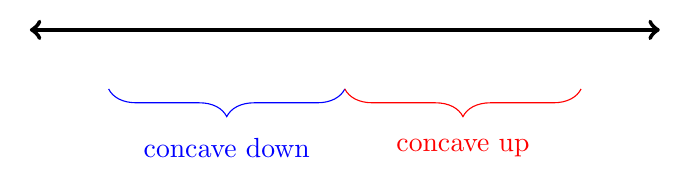
\begin{tikzpicture}
\draw[ultra thick, <->] (-4,0)--(4,0);
\YExcoord{0}{3}
\YExcoord{-3}{\textcolor{blue}{a}}
\YExcoord{3}{\textcolor{red}{b}}
\draw[decorate, decoration={brace, amplitude=10pt, mirror}, blue] (-3,-.75)--(0,-.75);
\draw[decorate, decoration={brace, amplitude=10pt, mirror}, red] (0,-.75)--(3,-.75);
\draw[blue] (-1.5,-1.5) node{concave down};
\draw[red] (1.5,-1.5) node{concave up};
\end{tikzpicture}

OR
\vspace{5mm}

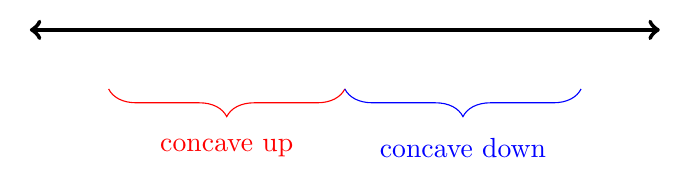
\begin{tikzpicture}
\draw[ultra thick, <->] (-4,0)--(4,0);
\YExcoord{0}{3}
\YExcoord{-3}{\textcolor{red}{b}}
\YExcoord{3}{\textcolor{blue}{a}}
\draw[decorate, decoration={brace, amplitude=10pt, mirror}, red] (-3,-.75)--(0,-.75);
\draw[decorate, decoration={brace, amplitude=10pt, mirror}, blue] (0,-.75)--(3,-.75);
\draw[red] (-1.5,-1.5) node{concave up};
\draw[blue] (1.5,-1.5) node{concave down};
\end{tikzpicture}
\end{center}

Since $f''(a)<0$ and $f''(b)>0$, and since $f''(x)$ is continuous, the Intermediate Value Theorem tells us that there exists some $x$ strictly between $a$ and $b$ with $f''(x)=0$. \textcolor{red}{So, we know $f''(x)=0$ somewhere between $a$ and $b$. The question is, where exactly could that be?}


\begin{itemize}
\item $f''(x)<0$ (and hence $f''(x) \neq 0$) for all $x$ between $a$ and 3
\item $f''(x)>0$ (and hence $f''(x) \neq 0$)  for all $x$ between $b$ and 3
\item So, any number between $a$ and $b$ that is not 3 has $f''(x)\neq 0$.
\end{itemize}So, $x=3$ is the only possible place between $a$ and $b$ where $f''(x)$ could be zero. Therefore, $f''(3)=0$.

Remark: this is why, in general, we set $f''(x)=0$ to find inflection points. (They can also occur where $f''(x)$ does not exist.)
\end{solution}
